\section{Administración de riesgos en un proyecto civil}

Existen tres categorías más importantes en la identificación de riesgos de proyectos IOC:
\begin{itemize}
    \item Riesgos de diseño
    \item Riesgos externos
    \item riesgos ambientales
    \item Riesgos organizacionales
    \item riesgos de administración de proyectos
    \item Riesgos legales y contractuales
    \item Riesgos de construcción
\end{itemize}

Estos riesgos se califican en función de su probabilidad de ocurrencia (del 1 al 5) y su impacto en el proyecto (del 1 al 5). La matriz de riesgos es una herramienta comúnmente utilizada para visualizar y priorizar estos riesgos.
A continuación, se presenta un ejemplo de una matriz de riesgos:
\begin{figure}[h]
    \centering
    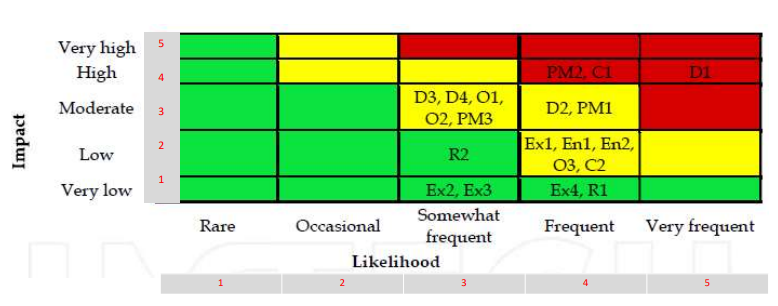
\includegraphics[width=0.8\textwidth]{Graficos/matriz.png}
    \caption{Matriz de riesgos de un proyecto IOC}
    \label{fig:matriz_riesgos}
\end{figure} 

Algunos ejemplos de riesgos que pueden surgir en un proyecto IOC son:
\begin{itemize}
    \item Riesgos de diseño: cambios en los requisitos del cliente, errores de diseño, falta de experiencia del equipo de diseño.
    \item Riesgos externos: cambios en la legislación, problemas con proveedores, condiciones climáticas adversas.
    \item Riesgos ambientales: contaminación del sitio, impacto en la fauna y flora local, problemas de salud pública.
    \item Riesgos organizacionales: falta de comunicación entre departamentos, conflictos internos, falta de recursos.
    \item Riesgos de administración de proyectos: falta de planificación adecuada, problemas con el cronograma, sobrecostos.
    \item Riesgos legales y contractuales: disputas contractuales, incumplimiento de normativas, problemas legales con terceros.
    \item Riesgos de construcción: accidentes laborales, problemas con subcontratistas, retrasos en la entrega de materiales.
\end{itemize}

También se puede hacer una matriz de evaluación de riesgos, que considera 7 factores:
\begin{itemize}
    \item Riesgo
    \item Repercusiones
    \item Probabilidad de que suceda
    \item Magnitud de las repercusiones
    \item Disparador de la acción 
    \item Responsable
    \item Plan de respuesta
\end{itemize}

Un ejemplo de matriz de evaluación de riesgos es el siguiente:
\begin{table}[h]
    \centering
    \small % Reduce tamaño de fuente
    \begin{tabularx}{\textwidth}{|c|X|c|c|X|c|X|}
        \hline
        \textbf{Riesgo} & \textbf{Repercusiones} & \textbf{Probabilidad} & \textbf{Magnitud} & \textbf{Disparador} & \textbf{Responsable} & \textbf{Plan de respuesta} \\
        \hline
        Clima adverso & + costos y retrasos & 3 & 4 & Pronóstico met. 2 días antes & Jefe de obra & Planificación de contingencias y ajustes al cronograma \\
        \hline
    \end{tabularx}
    \caption{Matriz de evaluación de riesgos}
\end{table}

Para poder calcular el riesgo se utiliza la siguiente fórmula:
\begin{equation}
    \text{Riesgo} = \text{Probabilidad} \times \text{Impacto}
\end{equation}
Si un riesgo tiene poca probabilidad y bajo impaccto, será capaz de aceparlo, pero si tiene alta probabilidad y alto impacto, se deberá prestar atención.

\section{Análisis de licitaciones, bases técnicas y contratos}

\subsection*{Etapa Inicial de un Proyecto OOCC}

\begin{itemize}
    \item Garantizar que el contratista/subcontratista comprenda los riesgos al hacer una oferta para un proyecto/servicio propuesto.
    \item El contratista/subcontratista puede incluir cantidades de reserva para contingencias en el precio de la oferta.
    \item El contratista/subcontratista puede desistir de presentar una oferta.
\end{itemize}

\subsection*{Criterios de Presentación de Presupuesto}

\begin{itemize}
    \item La oferta final se puede ver afectada por la estrategia que se haya tomado para la propuesta específica.
    \item El monto final puede bajar si el contratista tiene mucho interés en ganar el proyecto.
    \item El monto final puede subir si se tiene mucho trabajo en paralelo a este proyecto.
\end{itemize}

\subsection*{Decisión para Desarrollar una Propuesta}

\begin{itemize}
    \item La evaluación del contratista sobre la posibilidad de seguir o no con la preparación de una propuesta, en ocasiones se conoce como: \textbf{Decisión de Oferta / No Oferta}.
    \item Se pueden considerar los siguientes factores al decidir desarrollar una propuesta:
    \begin{itemize}
        \item Nuestras ventajas, fortalezas o capacidades diferenciadoras.
        \item Nuestras debilidades.
    \end{itemize}
\end{itemize}

\subsection*{Disminución / Mitigación de Riesgos}

\begin{itemize}
    \item Se pueden considerar los siguientes factores al decidir desarrollar una propuesta:
\end{itemize}

\begin{table}[h]
    \centering
    \small
    \begin{tabular}{|c|p{8cm}|c|p{4cm}|}
        \hline
        \textbf{N°} & \textbf{Factor} & \textbf{Puntuación (A/M/B)} & \textbf{Comentarios} \\
        \hline
        1 & Competencia & & \\
        \hline
        2 & Riesgo & & \\
        \hline
        3 & Consistencia con nuestra misión & & \\
        \hline
        4 & Oportunidad para ampliar nuestras capacidades & & \\
        \hline
        5 & Reputación con el cliente & & \\
        \hline
        6 & Disponibilidad de fondos & & \\
        \hline
        7 & Recursos disponibles para preparar propuesta de calidad & & \\
        \hline
        8 & Recursos disponibles para realizar el proyecto & & \\
        \hline
    \end{tabular}
    \caption{Planilla tipo de Lista de verificación de licitar/no licitar}
\end{table}

\noindent El \textbf{contratista} decidirá la acción de presentar su oferta:

\begin{center}
    \fbox{\textbf{Licitar \quad / \quad No Licitar}}
\end{center}

\subsection*{Factores que Influyen en la Decisión de Licitar / No Licitar}

\noindent Según un estudio, existen tres principales características de factores contribuyentes a la determinación final para licitar o no licitar en la industria de la construcción:

\begin{enumerate}
    \item Factores relacionados a la empresa,
    \item Factores relacionados al proyecto,
    \item Condiciones y expectativas del mercado, junto con consideraciones estratégicas.
\end{enumerate}

\noindent Estos factores pueden ser identificados:
\begin{itemize}
    \item Por el cliente, durante la etapa de elaboración de normativa o el llamado a propuesta (FRP) del proyecto.
    \item Por el contratista, durante la etapa de elaboración de su propuesta.
\end{itemize}

\noindent El \textbf{MANDANTE} decidirá acción de:
\begin{center}
    \fbox{\textbf{Adjudicar \quad / \quad No Adjudicar}}
\end{center}

\newpage
\section{Planificación y Gestión de Riesgos en Proyectos de Ingeniería Civil}

\subsection*{Evaluación de Riesgos}
Para manejar adecuadamente los riesgos en un proyecto, es necesario determinar:
\begin{itemize}
    \item La probabilidad de que ocurra cada riesgo.
    \item El impacto que tendría sobre los objetivos del proyecto.
\end{itemize}
Cada riesgo puede ser valorizado como alto, medio o bajo, o con valores numéricos(-1, 0, 1). Esto permite priorizar los riesgos según su probabilidad e impacto.

\subsection*{Plan de Respuesta ante Riesgos}
\begin{itemize}
    \item Se define un conjunto de acciones para evitar o reducir la probabilidad o el impacto de los riesgos.
    \item Cada riesgo debe tener un plan de acción y responsables asignados.
    \item Se utiliza una matriz de evaluación de riesgos como herramienta clave.
\end{itemize}

\subsection*{Implementación y Seguimiento}
\begin{itemize}
    \item Incluir reservas de contingencia en el presupuesto.
    \item Monitorear los riesgos identificados y detectar nuevos.
    \item Evaluar periódicamente la efectividad de las respuestas.
    \item Las reuniones de coordinación permiten actualizar los riesgos y documentar lecciones aprendidas.
\end{itemize}

\subsection*{Métodos de Identificación de Riesgos}
\begin{itemize}
    \item Lluvia de ideas con el equipo.
    \item Clasificación por categoría:
    \begin{itemize}
        \item Técnicos: nuevas tecnologías, estándares de calidad.
        \item Programación: retrasos de proveedores.
        \item Costo: variaciones por inflación o tiempo.
        \item Recursos Humanos: disponibilidad de personal.
        \item Externos: clima, regulación, stakeholders.
        \item Cliente: atrasos en pagos, aprobación de entregables.
    \end{itemize}
    \item Uso de experiencias aprendidas de proyectos anteriores.
\end{itemize}

\subsection*{Estimación de Impacto}
Por cada riesgo identificado se deben estimar los impactos potenciales:
\begin{itemize}
    \item Retrasos en el programa.
    \item Costos adicionales significativos.
    \item Riesgo de incumplimiento de especificaciones.
    \item Multas o penalizaciones contractuales.
\end{itemize}

\subsection*{Buenas Prácticas}
\begin{itemize}
    \item Asegurar una planificación detallada del alcance.
    \item Preparar paquetes de trabajo con anticipación.
    \item Revisar interferencias entre .
    \item Estimar correctamente la duración de actividades.
    \item Aplicar métodos como la ruta crítica (CPM).
    \item Hacer control y seguimiento continuo de los hitos.
\end{itemize}

\subsection*{Casos de Proyecto}
\begin{itemize}
    \item Instalación de torre grúa en obra.
    \item Diferencias de cubicación y su impacto económico.
    \item Generación y acumulación de residuos en faena.
\end{itemize}

\newpage
\section{Preguntas de Selección Múltiple y Respuestas Comentadas}

\subsection*{Pregunta 1}
\textbf{El material de video visto en clases Unidad 4, sobre análisis de riesgos dentro del sector construcción, analiza temas relacionados con:}
\begin{itemize}
    \item[A.] Criterios de Sustentabilidad en obras IOC
    \item[B.] Cambio de estrategia pública en obras de construcción
    \item[C.] \textbf{Riesgos compartidos en alza de precios de materiales entre cliente y contratista}
\end{itemize}

\textit{Comentario:} Esta fue la temática central del video de la Unidad 4, enfocado en cómo se abordan los riesgos financieros en contextos inflacionarios, destacando la importancia de compartir los riesgos contractuales.

\subsection*{Pregunta 2}
\textbf{¿A qué tipo de estudio de Evaluación Ambiental corresponde cuando el titular declara que el proyecto no generará ninguno de los efectos del Art. 11 de la Ley 19.300?}
\begin{itemize}
    \item[A.] \textbf{DIA (Declaración de Impacto Ambiental)} 
    \item[B.] EIA (Evaluación de Impacto Ambiental)
    \item[C.] Aplica realizar ambos estudios
\end{itemize}

\textit{Comentario:} La DIA es aplicable cuando se determina que el proyecto no produce efectos significativos. El EIA se requiere solo si alguno de los criterios del Art. 11 se ve afectado.

\subsection*{Pregunta 3}
\textbf{El método TVD (Target Value Design) contempla aplicar los siguientes criterios a la hora de abordar un proyecto de ingeniería:}
\begin{itemize}
    \item[A.] Todos los diseñadores se involucran desde el inicio
    \item[B.] El costo objetivo nunca debe ser excedido
    \item[C.] Compartir riesgos y recompensas
    \item[D.] \textbf{Todas las anteriores} 
\end{itemize}

\textit{Comentario:} Todos los ítems listados son principios fundamentales del TVD, el cual busca integración temprana, control de costos y colaboración entre actores del proyecto.

\subsection*{Pregunta 4}
\textbf{Dentro de Lean Construction, se indicó que uno de los desperdicios (mudas) que se presenta en tema de sobreproducción se refiere al exceso de materia prima, productos o procesos no en uso.}
\begin{itemize}
    \item[A.] \textbf{Verdadero}
    \item[B.] Falso
\end{itemize}

\textit{Comentario:} En Lean, la sobreproducción es uno de los ocho desperdicios. Generar más de lo necesario genera acumulación innecesaria, costos adicionales y uso ineficiente de recursos.

\section{Resolución de la Parte Teórica - Evaluación de Propuestas}

\subsection*{Cálculo de Nota Técnica}

La Oferta Técnica tiene una ponderación del 70\% y se compone de 5 criterios evaluados con un máximo de 80 puntos. Las ponderaciones específicas para cada criterio son:

\begin{center}
\begin{tabular}{|c|l|c|}
\hline
\textbf{Código} & \textbf{Criterio} & \textbf{Ponderación dentro de Nota Técnica (\%)} \\
\hline
X1 & Experiencia y antecedentes de la empresa & 25\% \\
X2 & Equipo de trabajo ofrecido               & 15\% \\
X3 & Seriedad de la oferta                    & 10\% \\
X4 & Capacidad económica                      & 20\% \\
X5 & Capacidad técnica                        & 30\% \\
\hline
\end{tabular}
\end{center}

Los puntajes por empresa son:

\begin{center}
\begin{tabular}{|c|c c c c c|}
\hline
\textbf{Empresa} & X1 & X2 & X3 & X4 & X5 \\
\hline
Empresa 1 & 55 & 35 & 70 & 20 & 80 \\
Empresa 2 & 45 & 65 & 65 & 50 & 70 \\
Empresa 3 & 35 & 45 & 55 & 45 & 55 \\
\hline
\end{tabular}
\end{center}

Aplicando las ponderaciones a cada empresa:

\begin{center}
\begin{tabular}{|c|c|}
\hline
\textbf{Empresa} & \textbf{Nota Técnica (70\%)} \\
\hline
Empresa 1 & $(55)(0.25) + (35)(0.15) + (70)(0.10) + (20)(0.20) + (80)(0.30) = 13.75 + 5.25 + 7.00 + 4.00 + 24.00 = \textbf{54.0}$ \\
Empresa 2 & $(45)(0.25) + (65)(0.15) + (65)(0.10) + (50)(0.20) + (70)(0.30) = 11.25 + 9.75 + 6.50 + 10.00 + 21.00 = \textbf{58.5}$ \\
Empresa 3 & $(35)(0.25) + (45)(0.15) + (55)(0.10) + (45)(0.20) + (55)(0.30) = 8.75 + 6.75 + 5.50 + 9.00 + 16.50 = \textbf{46.5}$ \\
\hline
\end{tabular}
\end{center}

\subsection*{Cálculo de Nota Económica}

Se asigna 80 puntos a la oferta más baja y se calcula el puntaje para las demás usando:

\[
\text{Puntaje empresa} = \left( \frac{\text{Oferta más baja}}{\text{Oferta empresa}} \right) \times 80
\]

\begin{itemize}
    \item Oferta más baja: Empresa 3 con 34.000 UF.
\end{itemize}

\begin{center}
\begin{tabular}{|c|c|c|}
\hline
\textbf{Empresa} & \textbf{Oferta Económica (UF)} & \textbf{Nota Económica (30\%)} \\
\hline
Empresa 1 & 35.500 & $\left(\frac{34000}{35500}\right) \times 80 = 76.5$ \\
Empresa 2 & 37.500 & $\left(\frac{34000}{37500}\right) \times 80 = 72.5$ \\
Empresa 3 & 34.000 & $80.0$ \\
\hline
\end{tabular}
\end{center}

\subsection*{Cálculo de Nota Final}

Se ponderan las notas técnica y económica:

\[
\text{Nota Final} = (\text{Nota Técnica}) \times 0.70 + (\text{Nota Económica}) \times 0.30
\]

\begin{center}
\begin{tabular}{|c|c|c|c|}
\hline
\textbf{Empresa} & \textbf{Nota Técnica (70\%)} & \textbf{Nota Económica (30\%)} & \textbf{Nota Final} \\
\hline
Empresa 1 & 54.0 & 76.5 & $(54)(0.70) + (76.5)(0.30) = 37.8 + 22.95 = \textbf{60.75}$ \\
Empresa 2 & 58.5 & 72.5 & $(58.5)(0.70) + (72.5)(0.30) = 40.95 + 21.75 = \textbf{62.7}$ \\
Empresa 3 & 46.5 & 80.0 & $(46.5)(0.70) + (80.0)(0.30) = 32.55 + 24.0 = \textbf{56.55}$ \\
\hline
\end{tabular}
\end{center}

\subsection*{Conclusión}

La propuesta se adjudica a la \textbf{Empresa 2}, ya que obtuvo la \textbf{mayor nota final} (62.7 puntos), producto de un buen equilibrio entre oferta técnica sólida y una oferta económica competitiva.


\section{Resolución Parte Teórica – Transferencia de Riesgos y Matriz de Evaluación}

\subsection*{2. Transferencia de Riesgos en Proyectos de Construcción}

Según el artículo \textit{"Risk Management in Construction Project"} revisado en clase, existen tres formas principales mediante las cuales un contratista puede transferir los riesgos en un proyecto de construcción:

\begin{enumerate}
    \item \textbf{Contratación de seguros:} 
    Utilizado para cubrir eventos fuera del control del contratista, como fenómenos climáticos extremos, robos, accidentes graves o fuerza mayor. Estos seguros permiten derivar la responsabilidad financiera a una aseguradora.

    \item \textbf{Subcontratación:}
    Delegar a terceros (subcontratistas) la ejecución de ciertas actividades específicas bajo condiciones definidas en contrato. Así, se transfieren riesgos como el cumplimiento de estándares de calidad, costos de materiales y cronogramas de ejecución.

    \item \textbf{Modificación de cláusulas contractuales:}
    Se establecen condiciones contractuales explícitas que distribuyen responsabilidades ante eventos específicos. Por ejemplo, en caso de alza de precios de materiales o trámites administrativos, se pueden definir cláusulas de riesgo compartido entre mandante y contratista.
\end{enumerate}

\vspace{0.3cm}

\subsection*{3. Análisis de Riesgos – Caso Rehabilitación de Pavimentos en Aeropuerto}

\textbf{Contexto:} \\
El proyecto consiste en la rehabilitación de losas de hormigón en la pista de aterrizaje del Aeropuerto Internacional Arturo Merino Benítez, en la Región Metropolitana. Este tipo de obras se realiza en zonas de alta criticidad operacional, bajo restricciones horarias estrictas, y con exigencias de calidad y precisión. Por lo tanto, gestionar adecuadamente los riesgos técnicos, logísticos y ambientales es esencial para el éxito del proyecto.

\vspace{0.3cm}

\subsubsection*{Riesgos Identificados y Cuantificación}

\begin{center}
\begin{tabular}{|c|p{8.2cm}|c|c|}
\hline
\textbf{ID} & \textbf{Riesgo} & \textbf{Probabilidad (1–5)} & \textbf{Impacto (1–5)} \\
\hline
A & Demora en el transporte de hormigón premezclado & 2 & 4 \\
B & Resistencia f’c del hormigón menor a la especificada en ensayo & 2 & 5 \\
C & Fisuras en las losas recién hormigonadas & 3 & 4 \\
D & Altas temperaturas durante ejecución y curado & 3 & 3 \\
E & Error en cubicación del volumen necesario de hormigón & 4 & 3 \\
F & Restricción horaria impide terminar colada a tiempo & 2 & 4 \\
G & Fallas en coordinación con torre de control / interrupciones operativas & 3 & 5 \\
H & Mal funcionamiento de maquinaria de colocación o vibrado & 2 & 4 \\
I & Ausencia o falla de moldajes en faena & 2 & 3 \\
\hline
\end{tabular}
\end{center}

\vspace{0.3cm}

\subsubsection*{Priorización de Riesgos}

Se consideran de prioridad alta los riesgos con mayor producto entre impacto y probabilidad.

\begin{center}
\begin{tabular}{|c|c|}
\hline
\textbf{Riesgos de Prioridad Alta} & B, C, G \\
\textbf{Riesgos de Prioridad Media-Alta} & A, D, E, F, H \\
\textbf{Riesgos de Prioridad Media o Baja} & I \\
\hline
\end{tabular}
\end{center}

\vspace{0.3cm}

\subsubsection*{Matriz de Evaluación de Riesgos (Ampliada)}

\begin{table}[H]
\centering
\resizebox{\textwidth}{!}{
\begin{tabular}{|c|p{5cm}|c|c|p{3cm}|p{2.5cm}|p{4cm}|}
\hline
\textbf{ID} & \textbf{Repercusiones} & \textbf{Prob.} & \textbf{Impacto} & \textbf{Disparador} & \textbf{Responsable} & \textbf{Plan de Respuesta} \\
\hline
A & Rechazo del hormigón o pérdida de trabajabilidad & 2 & 4 & Congestión en ruta de acceso & Jefe de Producción & Cambiar horario o ruta; prever camiones extra \\
\hline
B & Demolición y recarpetado por no alcanzar f’c & 2 & 5 & Ensayo a 3 días con baja resistencia & Jefe de Calidad & Aditivos acelerantes, uso de sensores para control temprano \\
\hline
C & Retrabajo por aparición de grietas post-curado & 3 & 4 & Inspección visual diaria & Supervisor de ejecución & Control estricto de curado y temperatura \\
\hline
D & Hormigón pierde trabajabilidad, fisuras por retracción & 3 & 3 & Temperatura ambiente sobre 30°C & Laboratorio & Añadir aditivos plastificantes y protección de losas \\
\hline
E & Sobras o déficit de hormigón, costos adicionales & 4 & 3 & Diferencia entre cubicación y pedido & Topógrafo/Jefe Obra & Revisar cubicación antes de cada jornada \\
\hline
F & Incompletitud de jornada por restricción horaria & 2 & 4 & Toque de queda operacional & Jefe de Producción & Reprogramar por bloques de faena + cuadrilla adicional \\
\hline
G & Paralización de obra por conflictos con tráfico aéreo & 3 & 5 & Cambio de prioridad operacional & Coordinador general & Planificar con torre de control; establecer ventanas horarias \\
\hline
H & Parálisis parcial por falla en equipos clave & 2 & 4 & Falla de equipo vibrador o mixer & Encargado de maquinaria & Mantención preventiva; backup de equipos críticos \\
\hline
I & Retardo de inicio por falta de moldajes & 2 & 3 & Revisión de check-list incompleto & Jefe de montaje & Revisar disponibilidad días antes, almacenamiento en obra \\
\hline
\end{tabular}
}
\caption{Matriz de evaluación de riesgos para rehabilitación de pavimentos en aeropuerto}
\end{table}


